%第2章:準備
 本章では、システム開発の進め方と、設計の工程で作成したUML図について説明する。

\subsection*{V字モデル\cite{kumikomi}}
ソフトウェアを開発する上では、適切な開発プロセスに沿って作業を進める必要がある。本研究では、開発プロセスのモデルの一つであるV字モデルを採用し、開発を進めた。このモデルを用いた場合の、各プロセスの進め方を図\ref{buiji}に示す。このモデルではテストを重視しており、図\ref{buiji}からもわかるように、左側にある分析や設計、実装のプロセスと、各テストの工程との対応が理解しやすく、検証の段階において、検証の対象とすべき範囲が把握しやすいという利点がある。例えば、要求分析に対してはシステムテストが配置され、実装に対しては単体テストが配置されている。これは、プログラム作成などの実装の正しさを単体テストによって確認し、要求分析の正しさをシステムテストで確認することを示している。そして右側のテストの各プロセスで不具合が見つかった場合には、左側の対応するプロセスに戻って修正を行うことになる。本研究でも、このような開発プロセスモデルの手順に沿い、必要に応じて、前のプロセスに立ち返りながら、運用に至るまでのプロセスを進めた。なお、本論文ではシステムテストと同じ意味を持つ言葉として、総合テストという言葉を用いている。

\begin{figure}[htbp]
	\centering
	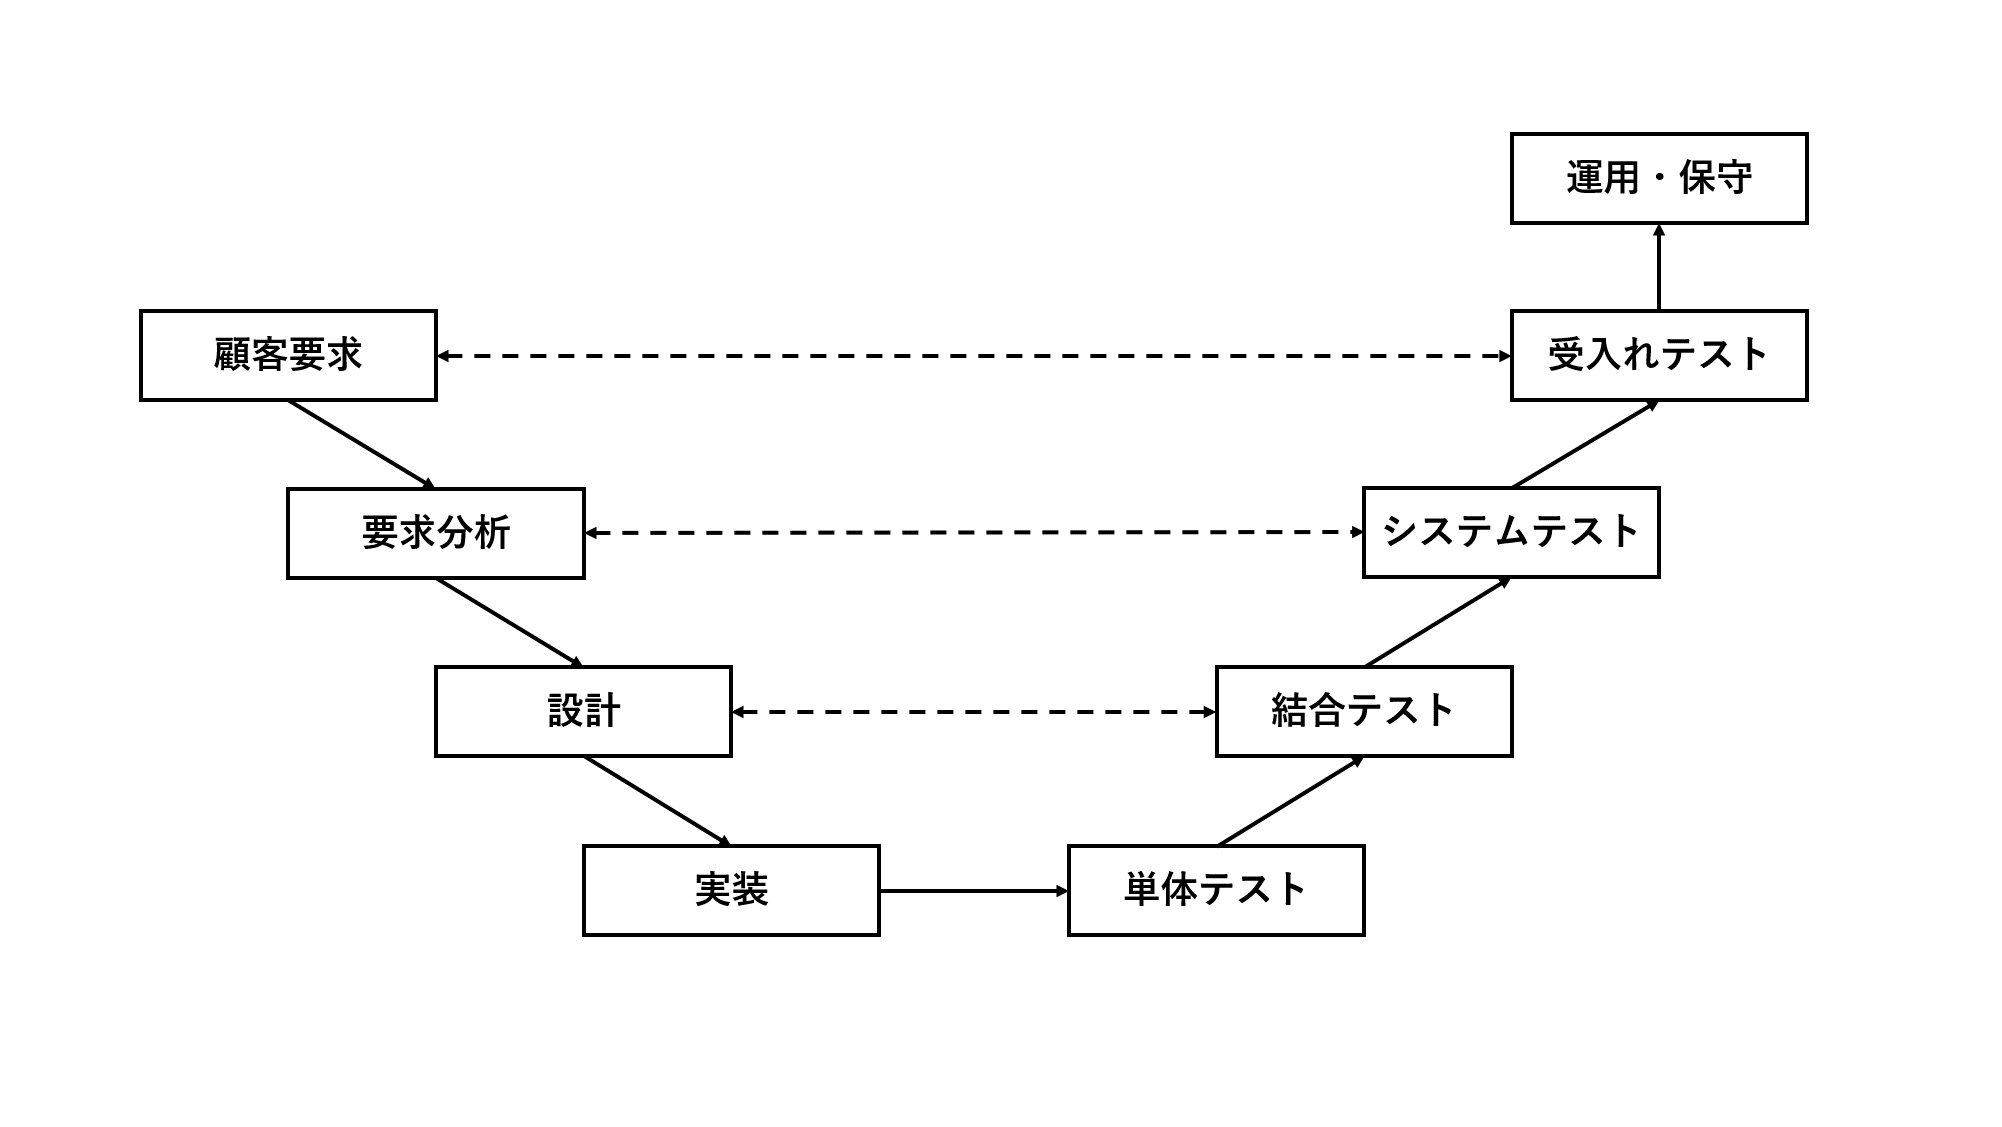
\includegraphics[width=12cm]{buiji.eps}
	\caption{V字モデル}
	\label{buiji}
\end{figure}


\subsection*{UML\cite{uml}}
UMLとは、統一モデリング言語(Unified Modeling Language)のことで、50以上の方法論やダイアグラム表記法のよさをできるだけ踏襲するように共通点を抽出すると同時に、オブジェクト指向でモデリングする際に必要な概念をすべて抽出し、それらを整理統合するような新たなモデル記述体系として考案されたものである。UMLを用いることで対象となる領域やシステムがどのような概念や要素から構成されているかという、構造的な側面のモデル化と、そうした概念や要素が時間経過の中でどのように相互作用して振る舞い、変化を行うかという動的な側面のモデル化の両方を、統一的でビジュアルな言語を使って行うことができる。そのため、組織やプロジェクト固有の慣習を捨象して世界共通の土台で議論できるようになり、計画やコンセプト作りから設計の詳細検討、実装やテストのための仕様定義といった様々な局面で普遍的に活用することができる。本研究でも、開発メンバー4人が1つのチームとして、共通認識を持って開発に取り組むため、要求分析・設計の工程でUML図を作成した。

\subsection*{ユースケース図\cite{uml}}
ユースケース図とは、システムがどのように機能すべきかという振る舞い(ユースケース)と、その外部環境(アクター)を表現するもので、システムの外部と内部との境界を明確にすることができる。ユースケース図を用いることで、エンドユーザの視点からシステムを見ることができ、エンドユーザや領域の専門家とのコミュニケーションが円滑になり、要求に対する相互の理解を保証することができるようになる。

\subsection*{アクティビティ図\cite{uml}}
 アクティビティ図とは、ひとまとまりの業務や処理の内容や流れを表すために、関連する複数の業務手順や処理ステップを順序だてて配置したもので、アクティビティ図によって、「企業全体や業務全体のモデルにおける一連のワークフロー」、「ユースケースごとに対応する処理フロー」、「あるオブジェクトの持つ1メソッドの内部のアルゴリズム」を記述することができる。

\subsection*{クラス図\cite{uml}}
クラス図とは、モデルの静的な構造を表現できる図であり、データ構造(属性リスト)と振る舞い(操作リスト)を持つクラスと、クラス間の静的な関係が表現できる。このクラス図が、UMLに代表されるオブジェクト指向分析設計における中心的な図となり、問題領域の構造や対象システムのアーキテクチャの静的な構成、システムの詳細設計、問題解決の発想の起点となる概念マップの構築といったことに広く用いることができる。

\subsection*{シーケンス図\cite{uml}}
シーケンス図とは、オブジェクト間のメッセージのやり取りを時系列に沿って並べて表現したもので、ユースケースを実現するのに必要なオブジェクトの集合と、その相互作用を明確に表現できる。ここでは、メッセージを時間順に1つずつ記述できるため、シナリオと対応させて具体的な内容を示す際に有用である。
